\section{Multicomponent heterogeneous systems}

After the study of systems where only one component was allowed we jumped to the study of multiple components having still one phase now also this last constraint has been released. Therefore, we want to understand how a general system behaves at thermodynamic equilibrium and to do that we need to start with the conditions for equilibrium itself. In fact, having now a series of possible phases and components the conditions seen in \eqref{eq:equiCond} are no longer exact, and we need to expand them as follows.
\thm{General equilibrium conditions}
{
    In a heterogeneous system with composed by $p$ phases and $c$ components we have that at equilibrium for every $\alpha$ and $\beta$ phases inside the system the following is true $\forall i \in \{0, \dots, c\}$ components
    \begin{equation}
        \label{eq:GenralEquilibriumConditions}
        T^\alpha = T^\beta, \hspace{2cm} P^\alpha = P^\beta, \hspace{2cm} \mu^\alpha_i = \mu^\beta_i. 
    \end{equation}
}
\pf{Proof}
{
    The proof is totally analogous to the one for the equilibrium conditions of the simpler case, the only difference is that now the differential of the internal energy contains more elements being
    \begin{equation}
        \dd U' = \sum_{\nu=1}^p\left( T^\nu \dd S'^\nu - P^\nu\dd V'^\nu + \sum_{i=1}^c \mu_i^\nu\dd n_i^\nu\right).
    \end{equation}
    Applying the equilibrium conditions of an isolated system that in our case are
    \begin{equation}
        \sum_\nu \dd U'^\nu = 0, \hspace{2cm} \sum_\nu \dd V'^\nu = 0, \hspace{2cm} \sum_\nu \dd n_i^\nu = 0,
    \end{equation}
    we can simply arrive to the wanted result.
}
\noindent
Basically, we need to keep in mind that more components are present and so, for two phases to be in equilibrium with each others we need that the chemical potentials of the different components are equal in both phases component by component.

The equilibrium conditions are the main general properties that are needed in order to study such systems. By keeping them in mind we can start to develop the theory of how this kind of general materials behave, understanding how the phases interacts with one another at equilibrium.

\subsection{Gibbs' phase rule}

In the construction of a phase diagram of a general system one may think that nothing is really known a priori due to the complexity of the system itself. Nevertheless, it's possible to find out some insight on at least the degrees of freedom that we have inside the diagram. In fact the equilibrium conditions gives large limitations on the possible thermodynamical variable that can change in certain regions of the phase diagram leaving us with the following result.
\thm{Gibbs' phase rule}
{
    In a system with $p$ phases and $c$ component the available degrees of freedom inside the system are given by the following relation
    \begin{equation}
        \label{eq:GibbsPhaseRule}
        f = c - P + 2.
    \end{equation}
}
\pf{Proof}
{
    We have, from \eqref{eq:GenralEquilibriumConditions}, that $T$ and $P$ must be the same for all phases, so $2$ variables are present. Then we also have the molar fractions $X_i^j$ to be possible variable having exactly $(c - 1)p$ of them, one for every component in every phase with a $-1$ due to the condition
    \begin{align}
        &\sum_i X^j_i = 1, &\forall j \in \{ 1, \dots, p \}.
    \end{align}
    Then we have the chemical potentials, which sets further restrictions to the system where we need to have all $\mu_i^1 = \dots = \mu_i^p$ for every component giving us $c(p-1)$ constrains which lead us to
    \begin{equation}
        f = 2 + (c-1)p - c(p-1) = c - p + 2,
    \end{equation}
    as expected.
}
\begin{figure}[t]
    \centering
    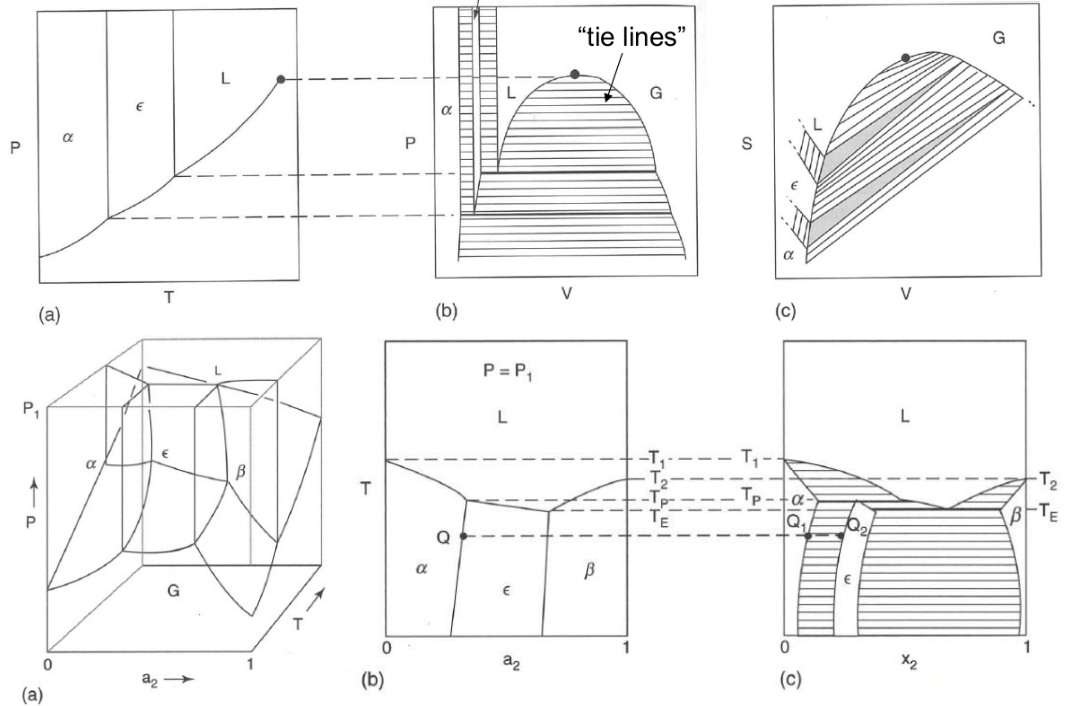
\includegraphics[width=0.8\textwidth]{Immagini/GeneralPhaseDiag.png}
    \caption
    {
        Examples of phase diagrams in different phase space for a two component, top, and a three component system, bottom. It's possible to see how the Gibbs' phase rule is respected perfectly in the $T$ vs $P$ phase space while modifications due to more freedom in the parameters are present in the others. In (b) of bottom row a isobaric section of (a) is represented.
    }
    \label{fig:GeneralPhaseDiag}
\end{figure}

\noindent
This rule is telling us a lot on the phase diagram properties in general. In fact, we can understand that in a system with two components if I want to have two phases coexist the degrees of freedom available becomes simply one, meaning that the region with two phases coexisting is a line as we know. Instead, if we want three phases zero degrees of freedom are present becoming a point, that is what we already called triple point. If we wanted to go up with the number of phases the value of $f$ will become negative, which is impossible, meaning that in a binary system only maximum three phases can coexist at once. The latter is a result that can be generalized really easily having that.
\cor{Maximum coexisting phases}
{
    In a system with $p$ phases and $c$ component the maximum number of coexisting phases are $c + 2$.
}
\noindent
Examples of this can be clearly seen inside \figref{fig:GeneralPhaseDiag} where phase diagrams of binary and ternary components are present, and we can see how in the formers the points find themselves in the connection of four phases the maximum number that can coexist.

It's also important to keep in mind that this result is valid as long as we represent the diagrams in the $(T, P)$ phase space, if we change visualization to another space the diagram will change and also the degrees of freedom can. Looking at the figure (b) in the top row of \figref{fig:GeneralPhaseDiag} we can see an example, substituting the variable $T$ with the volume $V$ makes it so that the latter can change at equilibrium since no condition on him is present inside \eqref{eq:GenralEquilibriumConditions}. Therefore, if we take a triple point and draw it on $(P,V)$ it will become a so-called \textbf{tie line} horizontal to the x-axis that allow to have the coexistence of the phases also while the volume of the system can change. That can also be seen for the $X_2$ case in the ternary component system of the bottom row where coexistent of different phases can be present at different values of molar content while in the normal representation they were points.

\subsection{Binary phase diagrams}

Let's now focus a moment on a binary heterogeneous system, a situation that we have already seen during the homogeneous study founding out that for certain interaction parameters and temperatures a miscibility gap appeared bringing the system to form two different phases. We want now to describe some features of this separation of phases using the same conceptual model used before, having that the homogeneous system separates in a phase $\alpha$ that is more rich of atoms of type $1$ and a $\beta$ rich of type $2$. Therefore, we are going to consider a system with a free energy of mixing as the one seen in \figref{fig:TwoPhase}, where it's possible to understand that the miscibility gap appear only in a certain range of temperature described by the parabola like shape found out in the phase diagram.
\begin{figure}[t]
    \centering
    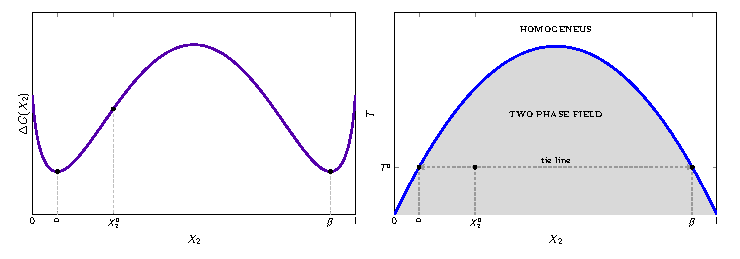
\includegraphics[width=\textwidth]{Immagini/TwoPhase.pdf}
    \caption
    {
        Illustration of a two phase system with miscibility gap, showing so a two phase field inside the phase diagram under the curve that describes the critical temperature of the system after which we have a homogeneous disordered phase. 
    }
    \label{fig:TwoPhase}
\end{figure}
The states inside that parabola forms the do called \textbf{two phase field}, meaning that inside those states it's possible for the system to form two phases to lower the total free energy. What we want to understand now is what changes from states that are on the same tie line of the two phase field.

To answer that question we can take a system with a certain molar fraction $X_2^0$ as depicted in \figref{fig:TwoPhase} and start thinking. The system will split, since it's in the two phase field, creating zones that are in a 1-rich state $\alpha$ and others in 2-rich state $\beta$. Nevertheless, the system has in total a major number of 1 type atoms since $X_2^0$ is lower than $0.5$ meaning that it will be able to create a larger number of $\alpha$ zones. Meaning that systems on different position on the tie line will differ by the \textbf{relative extensions of the two phases}, where systems more close to $\alpha$ will have larger 1-rich zones while the other will have larger $\beta$ phases rich of 2 type atoms. It's also possible to evaluate the weights $a_\alpha$ and $a_\beta$ of the two phases inside a system by using the following relations
\begin{align}
    &a_\alpha + a_\beta = 1, &a_\alpha X_2^\alpha + a_\beta X_2^\beta = X_2^0,
\end{align}
where $X_2^i$ represent the molar fractions of the two minima. These relations form a system of equation that can be easily solved obtaining the simple solutions
\begin{align}
    \label{eq:weightPhases}
    &a_\alpha = \frac{X_2^\beta - X_2^0}{X_2^\beta - X_2^\alpha}, &a_\beta = \frac{X_2^0 - X_2^\alpha}{X_2^\beta - X_2^\alpha}
\end{align}
In this way we can understand how much total volume of the system the two phases will take for themselves.

Another important thing that we say is that by now we have always looked at the free energy of mixing, but it's also interesting to look at the normal free energy of the system depicted in \figref{fig:DoubleTang}.
\begin{figure}[t]
    \centering
    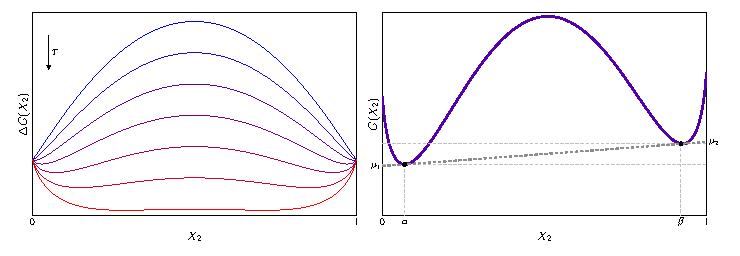
\includegraphics[width=\textwidth]{Immagini/DoubleTang.pdf}
    \caption
    {
        Representation of the mixing free energy at different temperatures on the left, and of the form of the normal free energy written as $G = \Delta G + \mu^0_2 X_2$ assuming $\mu^0_1 = 0$ on the left. It's possible to notice how the final form of $G$ is asymmetric.
    }
    \label{fig:DoubleTang}
\end{figure}
We know how the form of the free energy can be obtained from the mixing one by using the relation
\begin{equation}
    G = \Delta G + \sum_i \mu_i^0 X_i,
\end{equation}
with $\mu_i^0$ the chemical potential of the $i$-th component in its separated form. This makes so that the final form of the free energy is no more symmetric creating a variation of the chemical potentials respect to the one that we would expect from the \textbf{tangent construction} that we have discussed before. In fact, by taking the tangents in the two minima we would have that the chemical potentials obtained $\mu_i(X_2^\alpha)$ and $\mu_i(X_2^\beta)$ would be at different height and so have different values, while equilibrium conditions needed them to be equal. We can overcome this problem in a simple way, using the so-called \textbf{Double tangent construction}, where basically you construct a line connecting the two minima and the intercepts on the y-axis will give the $\mu_1$ on the left and $\mu_2$ on the right. Really simple and intuitive, even if we haven't demonstrated it mathematically, that allow us to find out $\mu$ also in this type of systems.